

\setcounter{section}{1}
\section{System Overview}
\bigskip

The Akriveia Beacon indoor locating rescue system combines hardware, electrical, and software systems to detect and locate multiple occupants within a building during an emergency disaster situation. Each individual component of the system is developed separately in the PoC (Proof of Concept) phase; then partially integrated in the Prototype phase and fully integrated in the Final Product phase. 

\bigskip
A high-level system overview presents three Locator Beacons, an ID tag, a data processing unit, and a graphical user interface (Figure \ref{sys_arch}). Using ultra-wideband (3.5-6.5GHz) wireless communication the Locator Beacons transmit signals to the ID tag to acquire a response. When the response returns back to the Beacon a time of flight measurement is acquired. The Time-of-Flight principle (\Gls{ToF}) is a method for measuring the distance between a sensor and an object, based on the time difference between the emission of a signal and its return to the sensor, after being reflected by an object. \cite{R2-0}. The ToF data will be forwarded to the portable data processing unit via a closed Wi-Fi network with \Gls{UDP}.  Then the processing unit will calculate the distance and coordinates of the ID tags using trilateration algorithm. Afterwards, the coordinates results are displayed on a GUI for operators.

\medskip
\begin{figure}[H]
\centering
    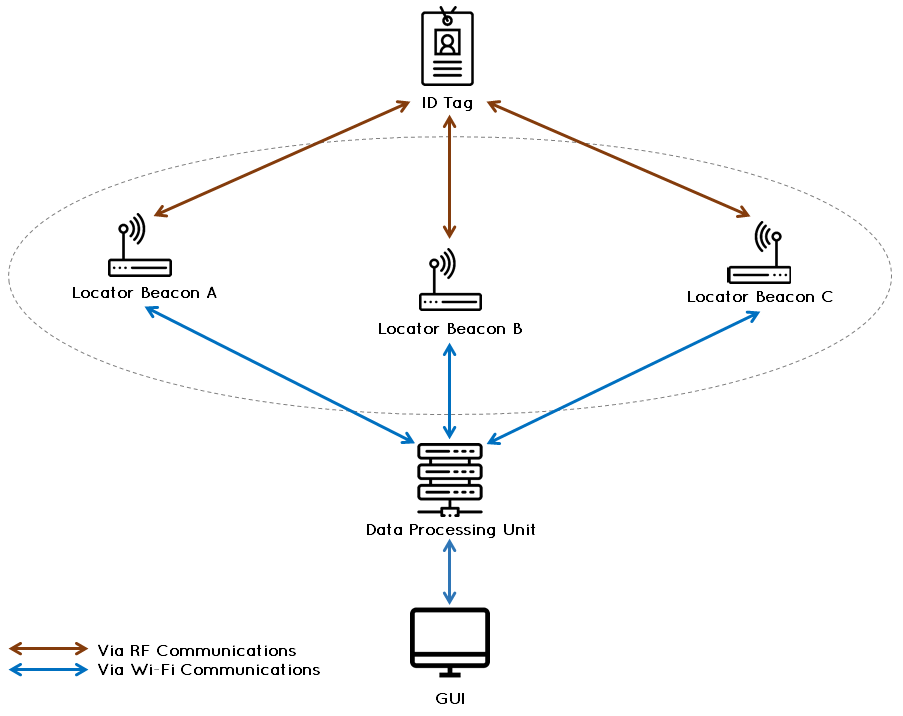
\includegraphics[scale=0.65]{./images/00_sys_arch.png}
    \caption{High Level System Layout}
    \label{sys_arch}
\end{figure}



\pagebreak
\subsection{Proof of Concept}
\medskip
The Proof of concept phase demonstrates the feasibility and functionality of an indoor location determination system. The \Gls{PoC} system will evaluate how effective the trilateration method is for determining the distance and location of a mobile ID tag in two dimensional space as well as to establish initial feasibility for the system. The PoC will be developed similar to the system block diagram shown in figure \ref{poc}.

\bigskip
ESP32 micro-controllers are used as the main controller units of the Beacon and ID Tags in PoC and further on. The ESP32 is an off the shelf, low-cost, low-power system on a chip micro-controllers with integrated WiFi and dual-mode Bluetooth. In the PoC, the system is designed to use Received Signal Strength Indicator (\Gls{RSSI}) from Bluetooth Low Energy (BLE) modules of the ESP32 to estimate distance between each beacon and ID tag. Each beacon determines the MAC address and a RSSI measurement from the advertising ID Tag and creates a data packet. The data packet is forwarded to the data processing unit - Raspberry Pi, via USB serial communications. The \Gls{RSSI} is then used to estimate distance between each ID Tag and the associating Beacon and the results of the trilateration method are output to a simple UI. 

\bigskip
\begin{figure}[H]
\centering
    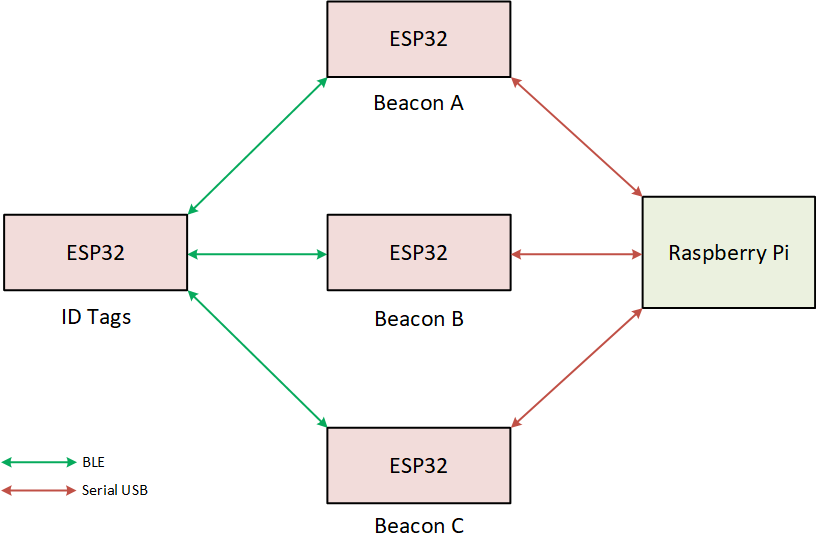
\includegraphics[width=\linewidth]{./images/01_poc.png}
    \caption{PoC System Block Diagram}
    \label{poc}
\end{figure}



\pagebreak
\subsection{Prototype}
\medskip
In the Prototype development phase the transceivers will be incorporated with Decawave DWM1000 UWB modules. The DWM1000 UWB uses radio frequencies in the range of 3.5 to 6.5GHz; this would significantly reduce issues of signal interference or multipath propagation which would occur by using RSSI with BLE. The DWM1000 will be incorporated as the transceiver with the ESP32 as the main MCU as shown in figure \ref{prototype} below. RF data communication functions will be established between four UWB modules with one as the ID Tag and three as the Locator Beacons to demonstrate distance estimation with DWM1000 UWB modules. This will be achieved by using signal fingerprinting to determine transmitter properties such as ToF and unique Tag identifier. Furthermore, trilateration algorithms will be implemented on data processing unit to determine near real time location and coordinates of ID Tags. Initial Implementation of software stack on the data processing unit and development of GUI will occur during this phase as well.

\bigskip
\begin{figure}[H]
\centering
    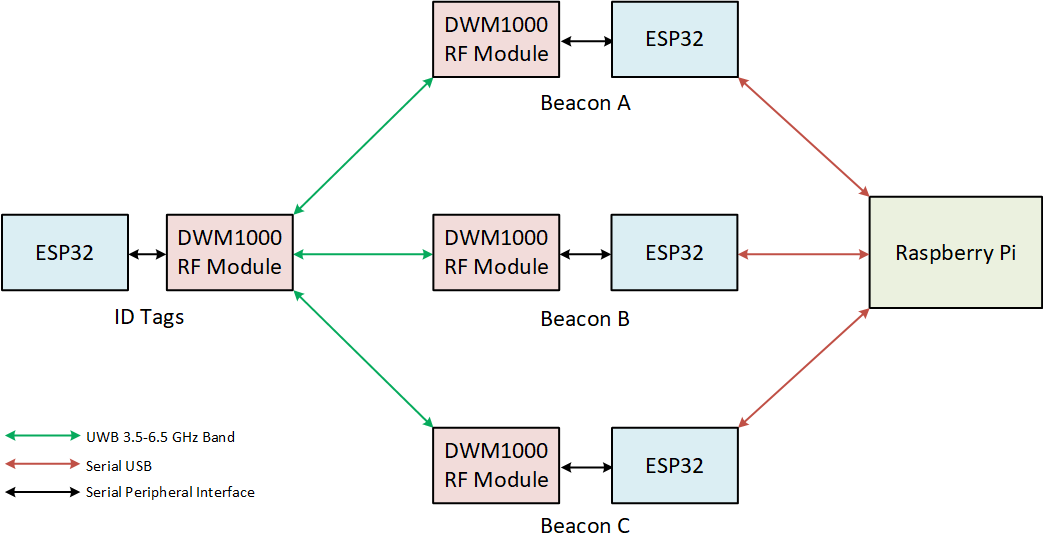
\includegraphics[width=\linewidth]{./images/02_prototype.png}
    \caption{Prototype System Block Diagram}
    \label{prototype}
\end{figure}


\pagebreak
\subsection{Final Product}
\medskip
The final product will demonstrate the fully functional indoor rescue system that detects the location of the ID tags and displays it accordingly on a GUI. Here the addition of ESP32’s WiFi modules for Beacon to DPU communications can be seen (Figure \ref{final}), as the Beacon will communicate via WiFi communication with the data processing unit. The WiFi network will be a closed private network meaning that the network is only share between beacons and the data processing unit to ensure security, reliability and stability. Furthermore, implementation of a RF harvesting circuit for charging the ID Tag device during deep sleep mode will occur throughout this stage. All the components of the systems will be fully integrated as a close-to-production product. Component circuits and \Gls{PCB} footprint will be minimized and proper casing will be made to house all electronics. The data processing unit will provide the user with a full GUI to interact with along with fully implemented features such as importable blueprints and system configurations.

\bigskip
\begin{figure}[H]
\centering
    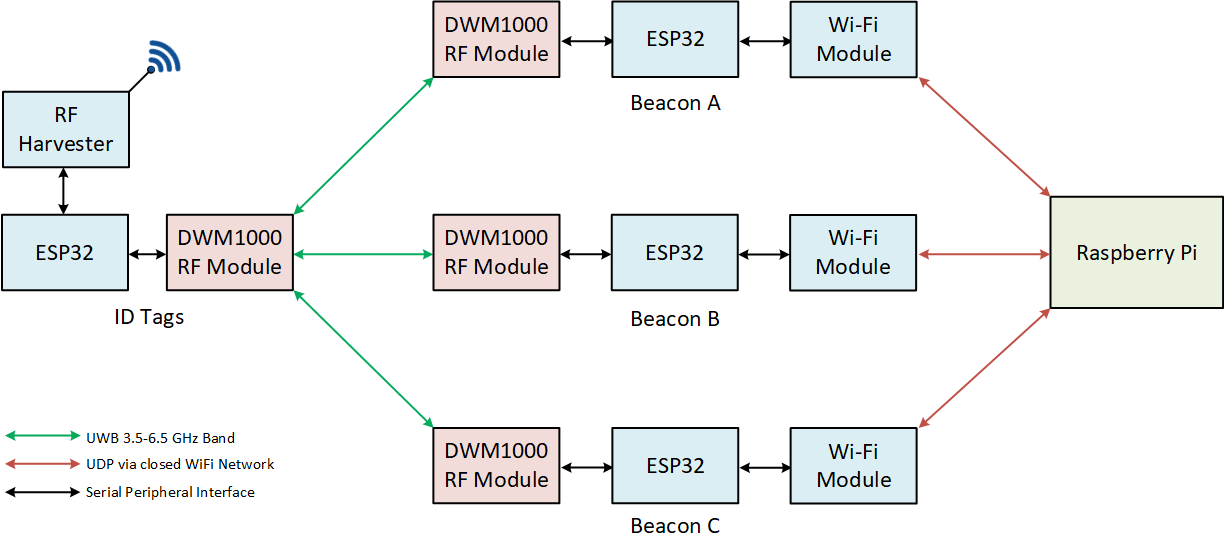
\includegraphics[width=\linewidth]{./images/03_final.png}
    \caption{Final System Block Diagram}
    \label{final}
\end{figure}


\pagebreak
\subsection{RF Fundamentals}
\medskip
Radio Frequencies (\Gls{RF}) is a common electromagnetic medium for communication systems to deliver digital information over the air from one point to another. Today, RF is used in many daily applications, such as \Gls{FM} radios and telecommunications. In fact, it is the discovery of RF signals that enables the deployment of many commercial wireless networks \cite{R2-4-1}.

\bigskip
On the electromagnetic spectrum, RF spans from 30Hz to 300GHz in frequency. More specifically, Bluetooth ranges from 2.40 to 2.48GHz and UWB ranges from 3.1 to 10.6GHz. RF has two main attributes: amplitude and frequency \cite{R2-4-1}. The amplitude represents the strength of an RF signal. The measurement of amplitude is power which indicates the amount of energy required for a signal to propagate over a given distance. The amplitude of an RF signal is susceptible to degradation as it travels over a distance in air \cite{R2-4-1}. The rate at which an RF signal degrades follows the inverse square law shown in Figure \ref{isl} , which states that generally signal strength decreases exponentially as distance increases. In theory, the degree of strength loss can be mitigated by having a more powerful signal to begin with provided that there is minimal obstacle against the signal on the way to its destination \cite{R2-4-2}.

\medskip
\begin{figure}[H]
\centering
    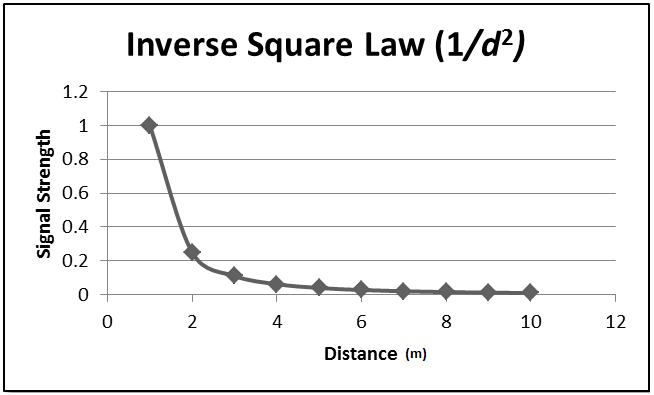
\includegraphics[scale=0.8]{./images/ISL.png}
    \caption{Relationship Between Signal Strength and Distance}
    \label{isl}
\end{figure}


\medskip
Another factor of RF that influences distance propagation is signal frequency. In RF, frequency describes the number of signal repetition per second. RF frequency is measured in Hertz (Hz), which is the number of cycles occurring each second. For instance, an RF radio operating at 2.4GHz means that the signal includes 2,400,000,000 cycles per second \cite{R2-4-1}. The effects of different frequencies on distance propagation is illustrated in a Free Space Path Loss graph shown in Figure \ref{fsp} below. The graph shows that there is positive correlation between signal strength degradation and frequency, where the higher the frequency, the more quickly signal-strength falls over distance \cite{R2-4-2}. In fact, this relationship is reasonable since the higher the frequency of a signal, the lower its wavelength. 

\medskip
\begin{figure}[H]
\centering
    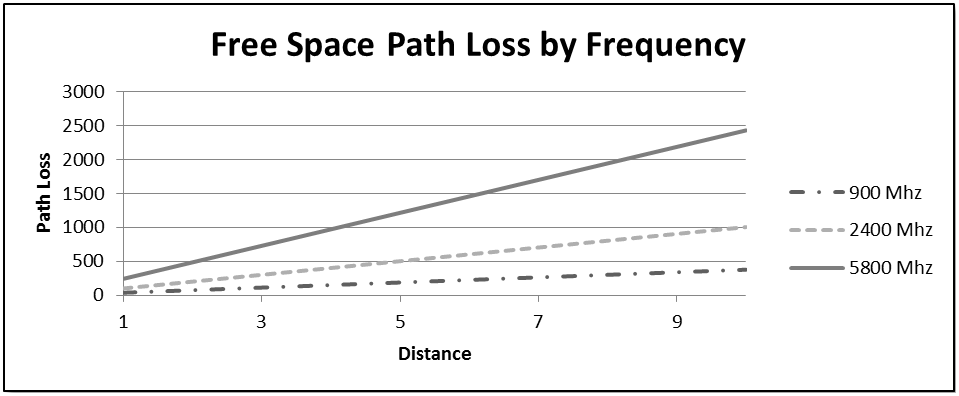
\includegraphics[width=\linewidth]{./images/FSP.png}
    \caption{Effects of Different Frequencies on Distance Propagation}
    \label{fsp}
\end{figure}

\medskip
Besides RF signal attributes, environmental factors can also influence the integrity of an RF signal. Multipath is one of the most common and inevitable factor that can delay and distort a travelling RF signal. Mutipath propogation is a phenomenon where an RF signal takes different paths when propagating from the source to the destination. As illustrated in Figure \ref{multipath}, contact with surfaces such as a desk or a ceiling contribute to the division of a signal into multiple signal portions to arrive at the destination at different times. This induces another phenomenon called multipath delay which causes the distortion of a signal's information. Since a signal is arriving as components, the receiver will not be able to interpret the information of the original signal during demodulation \cite{R2-4-1}.

\medskip
\begin{figure}[H]
\centering
    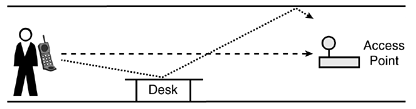
\includegraphics[scale=1.2]{./images/multipath.png}
    \caption{An Example of Multipath}
    \label{multipath}
\end{figure}

\pagebreak
\subsection{Received Signal Strength Indicator}
\medskip
Received Signal Strength Indicator, or RSSI describes the amount of power detected by the receiver during the reception of a packet. It is a metric measured in dBm and can be acquired through BLE API of the ESP32 module. Signal strength is influenced by the inverse square law from the previous section, which states that signal strength decreases exponentially as the distance from the transmitter increases, hence it is possible to estimate the proximity of the receiver from the transmitter based on the changes in measured RSSI value. The distance conversion formula from RSSI to distance is shown below. In the PoC phase, Akriveia uses RSSI as the distance-related metric \cite{R2-5-1}.

\medskip
\begin{equation*}
    Distance = 10^{(Measured\_Power - RSSI)/(10*N)}
\end{equation*}

\medskip
Measured power is the expected RSSI at a distance of one meter. This constant value can be acquired by calibration through averaging sufficient number of RSSI values between transceivers placed at one meter apart \cite{R2-5-3}.

\bigskip
N, is the environmental factor constant that ranges from values 2 to 4. It is a value set to adapt to the degree of indoor attenuation, interference and multipath \cite{R2-5-3}.

\medskip
\subsection{Ultra-Wideband and Time-of-Flight}
\medskip
Time of flight, or ToF is a distance related metric that describes the propagation time of a radio signal between a sender and a receiver. Precisely, it is the time it takes for a radio signal to travel from a sender to receiver and back to the sender. Since radio waves are a type of electromagnetic radiation, the travel speed of a radio signal is the speed of light, which is approximately thirty centimeters per nanosecond. Given the speed of light constant and a ToF value, the distance between a sender and a receiver can be computed using the Distance Speed Time formula as shown below \cite{R2-5-1}. To measure ToF in the nanosecond scale, Akriveia will employ the Ultra-Wideband (UWB) technology by using the DWM1000 module in the prototype and final product phase.

\medskip
\begin{equation*}
    Distance = Speed\:of\:light * ToF
\end{equation*}

\medskip
In narrowband systems, measuring signal arrival times with accuracy is a difficult task without complex algorithms. Due to bandwidth limitations, radios in narrowband systems cannot resolve signals influenced by multipath and may assume all received subpath signals arrived at the same time \cite{R2-5-2}. Fortunately, multipath components can be resolved using UWB radios due to larger signal bandwidth. UWB radios are formerly known as pulse radios as they send signals in short bursts called chips. The chips are radio energy pulses that carry information over a large bandwidth to counter the effects of multipath fading and interference that are present in conventional narrowband signals such as 2.4G/5G WiFi. Due to the short duration of chips, the effects of multipath are also received as echoes that do not interfere with the original signal \cite{R2-5-1}. As a result, UWB provides a great solution to indoor localization by allowing high precision ToF measuring capabilities.



\pagebreak
\subsection{Trilateration Methods}
\medskip
The Akriveia 2-D indoor localization solution determines the x-y coordinates of ID tags by trilateration. The method follows a lateration scheme with absolute distances, which uses distance-related metrics such as RSSI or ToF to determine the distance between a sender and a receiver. In the case where there is a single beacon and ID tag, the distance between the two entities can be interpreted as the radius of a circle traced with the beacon centered as shown in figure \ref{tri}. 

\begin{figure}[H]
\centering
    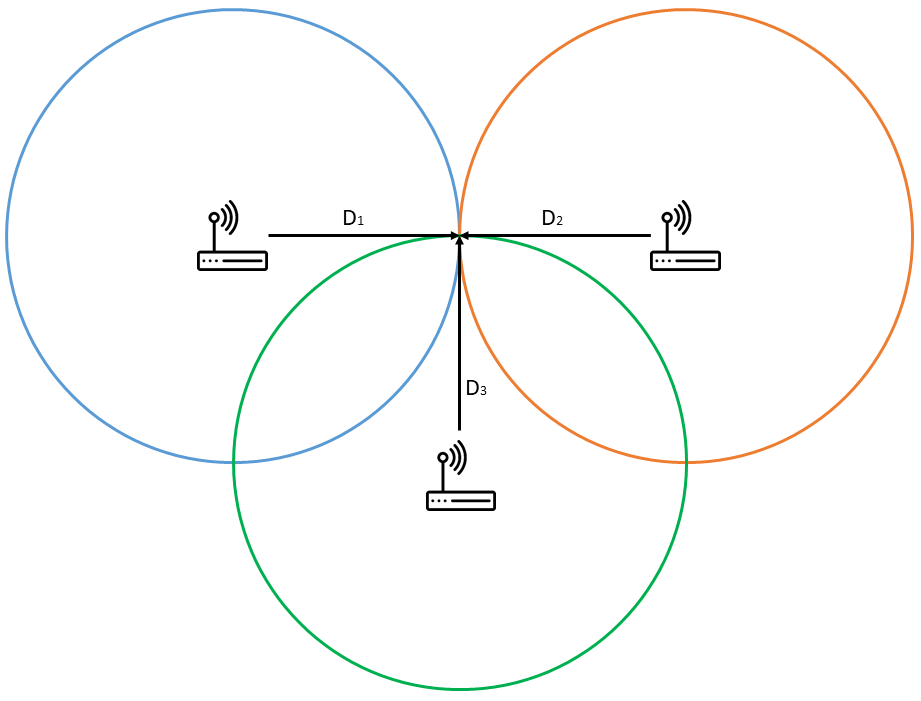
\includegraphics[scale=0.5]{./images/Tri.png}
    \caption{Trilateration Diagram}
    \label{tri}
\end{figure}
\medskip

Such a circle takes on a standard mathematical form as shown in the equation below, where the variables $x_0$ and $y_0$ are the 2-D coordinates of the beacon position relative to its environment, and $r_0$ is the distance between the beacon and the ID tag. 

\medskip
\begin{equation*}
	(x-x_{0})^2 + (y-y_{0})^2 = r_{0}^2
\end{equation*}

\medskip
The same concept applies to the scenario with three beacons and an ID tag. Given the 2-D coordinates the three beacons and their individual distance with respect to the ID tag, three circles can be traced to form an intersection point at the location of the ID tag. Hence, three standard form circle equations are generated to form a system of equations with two unknowns as shown below. The solution to the unknowns, or the intersection coordinates of the ID tag can be obtained by solving such a system.


\begin{equation*}
	(x-x_1)^2 + (y-y_1)^2 = {r_1}^2 
\end{equation*}
\begin{equation*}
	(x-x_2)^2 + (y-y_2)^2 = {r_2}^2 
\end{equation*}
\begin{equation*}
	(x-x_3)^2 + (y-y_3)^2 = {r_3}^2  
\end{equation*}

\pagebreak
The system of three equations can be ultimately simplified to the two equations shown below by expanding and equation elimination,

\begin{equation*}
	Ax + By = C
\end{equation*}
\begin{equation*}
	Dx + Ey = F
\end{equation*}

\medskip
where the representation of constants A, B, C, D, E and F are as follows,

\begin{equation*}
	A = -2x_1 + 2x_2
\end{equation*}
\begin{equation*}
	B = -2y_1 + 2y_2
\end{equation*}
\begin{equation*}
	C = {r_1}^2 - {r_2}^2 - {x_1}^2 + {x_2}^2 - {y_1}^2 + {y_2}^2
\end{equation*}
\begin{equation*}
	D = -2x_2 + 2x_3
\end{equation*}
\begin{equation*}
	E = -2y_2 + 2y_3
\end{equation*}
\begin{equation*}
	F = {r_2}^2 - {r_3}^2 - {x_2}^2 + {x_3}^2 - {y_2}^2 + {y_3}^2
\end{equation*}

\medskip
The system of two equations and two unknowns has the solution as shown below for the 2-D coordinates of an ID tag.

\begin{equation*}
	x = \frac{CE - FB} {EA - BD}
\end{equation*}
\begin{equation*}
	y = \frac{CD - AF} {BD - AE}
\end{equation*}


\pagebreak
\subsection{System Design Specification}
\medskip
The Akriveia Beacon consists of three main components: the Beacons, ID Tags, and the Data processing unit. The detailed specifications for each system will be outlined in their corresponding sections throughout the document. General system and performance specifications of Akriveia Beacon are listed in the table below.
\medskip
\bgroup
\def\arraystretch{1.5}
\begin{table}[H]
\centering
\begin{tabular}{ | m{3cm} | m{12.5cm} |}
\hline
\textbf{REQ.SY.1 - C} & The system must have two access modes: Emergency (for first responders), and Admin (for IT services)\\
\hline
\textbf{REQ.SY.2 - P} & Beacons and ID Tag must communicate with each other using BLE\\
\hline
\textbf{REQ.SY.3 - P} & Administrator must be able to access the system to perform health checks on the Beacons and ID tags \\
\hline
\textbf{REQ.SY.4 - P} & Administrator must be able to access the system to add/remove ID tags in the system database \\
\hline
\textbf{REQ.SY.5 - P} & The Beacons must use a WiFi mesh for forwarding data to DPU\\
\hline
\textbf{REQ.SY.6 - P} & The Beacons must contain a rolling buffer for ToF data for each id tag transmitted to\\
\hline
\textbf{REQ.SY.7 - P} & Each Beacons must use median of previous 10 samples of ToF data to sent to data processing unit\\
\hline
\textbf{REQ.SY.8 - P} & Beacons and ID Tag must communicate with each other using UWB (3.5-6.5GHz)\\
\hline
\textbf{REQ.SY.9 - F} & The System shall be easy to set up and tear down\\
\hline
\textbf{REQ.SY.10 - F} & The System must remain operational during/after small scale disasters such a small fires and earthquakes with magnitude less than 6.9\\
\hline
\end{tabular}
\caption{System Design Specification}
\end{table}
















